\documentclass[10pt]{article}

%\usepackage{revnum}

\usepackage{fancyhdr}
\usepackage{amsmath,amssymb,amsfonts}
\usepackage{graphicx}
\usepackage[utf8]{inputenc}
\usepackage{hyperref}
\usepackage{subfig}
\usepackage{fontawesome}

\oddsidemargin  0.25in
\evensidemargin 0.25in
\textwidth      6.3in
\topmargin      -0.25in
\textheight     8.7in
\parskip        0.1in
\parindent      0.0in

\hyphenation{}

\begin{document}
	
	\begin{center}
		{\huge Juan Irving Vasquez Gomez}
		\vspace{0.5cm}
		
		\begin{minipage}[b]{0.3\linewidth}
			\centering
			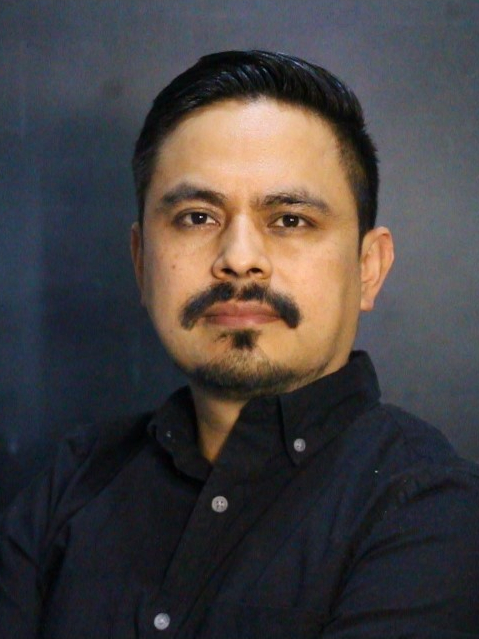
\includegraphics[width=\textwidth]{jivg36}
			%	\caption{default}
			%	\label{fig:figure1}
		\end{minipage}
		\hspace{0.5cm}
		\begin{minipage}[b]{0.6\linewidth}
			\textbf{Date of birth:} November, 1984 \\
			\textbf{Position:} Associate professor at Instituto Politécnico Nacional (IPN), Mexico.
			Centro de Innovación y Desarrollo Tecnológico en Cómputo (CIDETEC) \\ 
			\textbf{Address:} Av."Juan de Dios Bátiz" s/n esq. Miguel Othón de Mendizábal, 
			Col. Nueva Industrial Vallejo, Del. Gustavo A. Madero, Ciudad de México, C.P. 07700. \\
			\textbf{Telephone \faPhone:} +52 55 5729-6000 Ext. 52516. \\
			\textbf{e-mail \faEnvelopeO:} jvasquezg[at]ipn.mx, jirvingvg[at]gmail.com\\
			\textbf{URL \faExternalLink:} \url{https://jivg.org} \\
			\textbf{ORCID:} \url{https://orcid.org/0000-0001-8427-9333} \\
			\textbf{Scopus Id:} \href{https://www.scopus.com/authid/detail.uri?authorId=54415023500}{54415023500}\\
			\textbf{github \faGithub :} \url{https://github.com/irvingvasquez} \\
			\textbf{Kaggle:} \url{https://www.kaggle.com/irvingvasquez}
		\end{minipage}
			
	\end{center}


\begin{center}
{\bf Research Interests:} \\ Robotics, Computer Vision, Three-dimensional Modelling, Motion Planning.
\end{center}

\begin{itemize}

\item{\bf PERSONAL STATEMENT:}
	
I am a scientific researcher passionate about understanding the motion planning algorithms that involve active sensing. My training as an engineer and scientist has allowed me to propose, analyze and implement state-of-the-art solutions for several theoretical and practical problems. My current research interests include deep learning-based computer vision, robot motion planning, autonomous 3D reconstruction, and autonomous surface inspection.
	
\item{\bf EDUCATION:}

\begin{minipage}{1.5 in}
	2014\\
\end{minipage}
\begin{minipage}{4.5in}
	\textbf{PhD. in Computer Sciencies.} \textit{Institute for Astrophysics Optics and
	Electronics (INAOE) \href{https://www.inaoep.mx/}{\faExternalLink}.} Thesis: View Planning for 3D Object Reconstruction with Mobile Robots \href{https://jivasquez.files.wordpress.com/2015/03/tesis-doctorado.pdf}{\faFilePdfO}. Advisors: Enrique Sucar and Rafael Murrieta.\\ 
\end{minipage}


\begin{minipage}{1.5 in}
	2009\\
\end{minipage}
\begin{minipage}{4.5in}
	\textbf{M. Sc. in Computer Sciencies.} \textit{Institute for Astrophysics Optics and
		Electronics (INAOE) \href{https://www.inaoep.mx/}{\faExternalLink}.} Thesis: View Planning for Three-dimensional Object Reconstruction \href{https://jivasquez.files.wordpress.com/2015/03/tesis-maestria.pdf}{\faFilePdfO}. Advisors: Enrique Sucar and Efrain Lopez-Damian.\\ 
\end{minipage}

\begin{minipage}{1.5 in}
	2006\\
\end{minipage}
\begin{minipage}{4.5in}
	\textbf{B.S.E. in Computer Systems Engineering} \textit{Tehuacan Institute of Technology (ITT)}, Graduated by ``Score of excelence".\\ 
\end{minipage}

%\item {\bf PROFESSIONAL EXPERIENCE:} \\\\
%
%\begin{minipage}{1.5 in}
%	02/2016 - Current\\
%\end{minipage}
%\begin{minipage}{4.5in}
%	CONACYT Research Fellow assigned to Instituto Politécnico Nacional (IPN), Centro de Innovación y Desarrollo Tecnológico en Cómputo (CIDETEC). Project 1507.\\ 
%\end{minipage}
%
%%\begin{minipage}{1.5 in}
%%	01/2015 - 12/2015\\
%%\end{minipage}
%%\begin{minipage}{4.5in}
%%	CONACYT Research Fellow assigned to Instituto Politécnico Nacional, Centro de Innovación y Desarrollo Tecnológico en Cómputo. Project 1507.\\ 
%%\end{minipage}
%
%\begin{minipage}{1.5 in}
%08/2009 - 08/2014\\
%\end{minipage}
%\begin{minipage}{4.5in}
%Researcher and programmer for the INAOE's Markovito Team at the Robocup@home
%Competition.\\ 
%\end{minipage}
%
%\item{\bf MAIN AWARDS AND DISTINCTIONS}
%%

\begin{minipage}{1.5 in}
	2017 - 2019\\
\end{minipage}
\begin{minipage}{4.5in}
	Candidato a Investigador Nacional otorgado por el Consejo Nacional de Ciencia y Tecnología, México\\ 
\end{minipage}

\begin{minipage}{1.5 in}
	2020 - 2022\\
\end{minipage}
\begin{minipage}{4.5in}
	Investigador Nacional Nivel 1 otorgado por el Consejo Nacional de Ciencia y Tecnología, México\\ 
\end{minipage}
%
\item {\bf PUBLICATIONS:} \\

\begin{figure}[t]
	\subfloat[Publications distribution.\label{subfig-1:dummy}]{%
		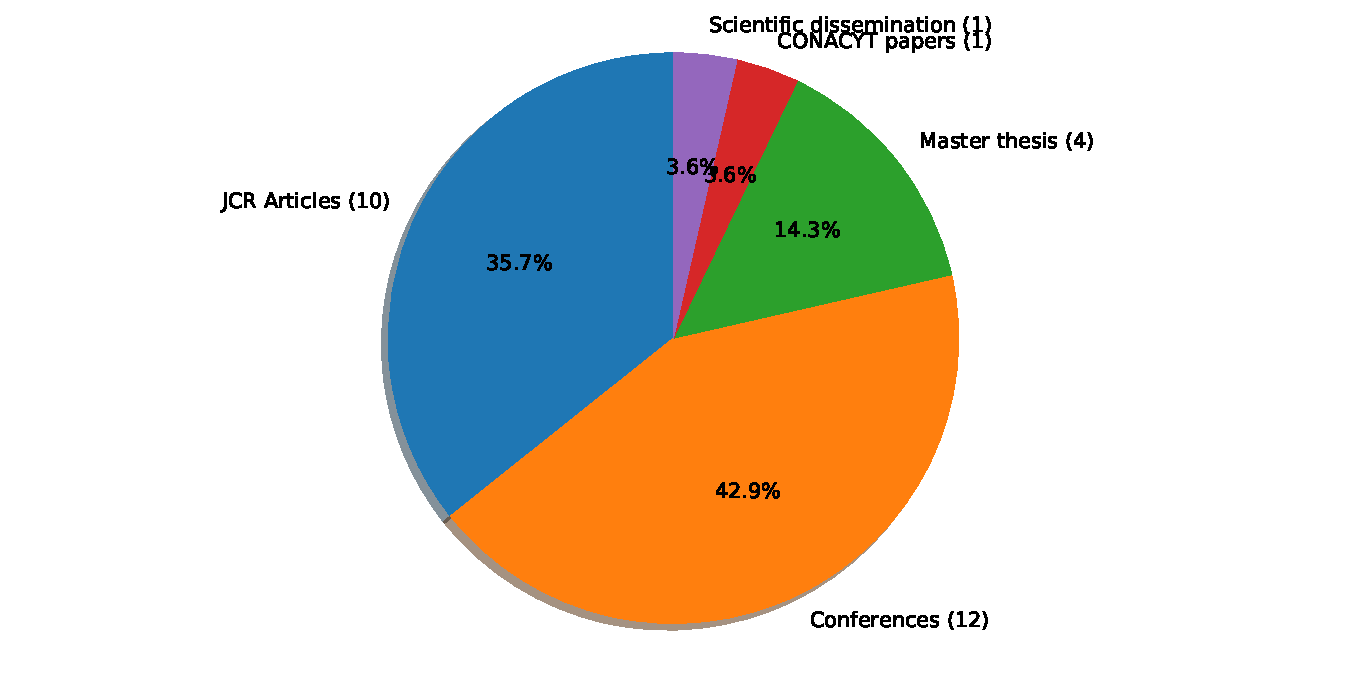
\includegraphics[trim=90 0 90 0, clip, width=0.60\textwidth]{../text/products_en.pdf}
	}
	\hfill
	\subfloat[Scopus metrics\label{subfig-2:dummy}]{%
		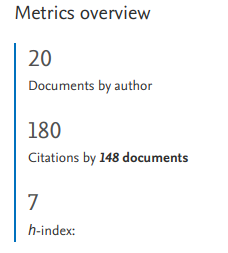
\includegraphics[width=0.35\textwidth]{../text/scopus_metrics.png}
	}
	\caption{Scientific products.}
	\label{fig:dummy}
\end{figure}

\begin{itemize}
	\item \textbf{JCR Journals}:
	\begin{itemize} 
\item L{\'o}pez-Jim{\'e}nez, Efren and Vasquez-Gomez, Juan Irving and Sanchez-Acevedo, Miguel Angel and Herrera-Lozada, Juan Carlos and Uriarte-Arcia, Abril Valeria, Columnar cactus recognition in aerial images using a deep learning approach,\textit{ Ecological Informatics,} (2019), I.F. 2.310 
\item Vasquez-Gomez, Juan Irving and Marciano-Melchor, Magdalena and Valentin, Luis and Herrera-Lozada, Juan Carlos, Coverage Path Planning for 2D Convex Regions,\textit{ Journal of Intelligent and Robotic Systems,} (2019), I.F. 2.020 
\item Vasquez-Gomez, J Irving and Sucar, L Enrique and Murrieta-Cid, Rafael and Herrera-Lozada, Juan-Carlos, Tree-based search of the next best view/state for three-dimensional object reconstruction,\textit{ International Journal of Advanced Robotic Systems,} (2018), I.F. 1.223 
\item Yervilla-Herrera, Heikel and Vasquez-Gomez, J Irving and Murrieta-Cid, Rafael and Becerra, Israel and Sucar, L Enrique, Optimal motion planning and stopping test for 3-D object reconstruction,\textit{ Intelligent Service Robotics,} (2018), I.F. 1.346 
\item Vasquez-Gomez, J Irving and Sucar, L Enrique and Murrieta-Cid, Rafael, View/state planning for three-dimensional object reconstruction under uncertainty,\textit{ Autonomous Robots,} (2017), I.F. 2.244 
\item Vasquez-Gomez, J Irving and Sucar, L Enrique and Murrieta-Cid, Rafael and Lopez-Damian, Efrain, Volumetric next-best-view planning for 3d object reconstruction with positioning error,\textit{ International Journal of Advanced Robotic Systems,} (2014), I.F. 0.526 
\end{itemize} 

	
	\item \textbf{Conferences}:
	\begin{itemize} 
\item Rodr{\'\i}guez-Hernandez, Erick and Vasquez-Gomez, Juan Irving and Herrera-Lozada, Juan Carlos, Flying through Gates using a Behavioral Cloning Approach, \textit{ 2019 International Conference on Unmanned Aircraft Systems (ICUAS),} 2019 
\item Vasquez-Gomez, Juan Irving and Herrera-Lozada, Juan-Carlos and Olguin-Carbajal, Mauricio, Coverage path planning for surveying disjoint areas, \textit{ 2018 International Conference on Unmanned Aircraft Systems (ICUAS),} 2018 
\item Vasquez-Gomez, Juan Irving and Herrera-Lozada, Juan Carlos and Olguin-Carbajal, Mauricio, Spatial resolution optimization for terrain coverage with UAVs, \textit{ 2017 International Conference on Mechatronics, Electronics and Automotive Engineering (ICMEAE),} 2017 
\item Vasquez-Gomez, Juan Irving and Melchor, Magdalena Marciano and Lozada, Juan Carlos Herrera, Optimal coverage path planning based on the rotating calipers algorithm, \textit{ 2017 International Conference on Mechatronics, Electronics and Automotive Engineering (ICMEAE),} 2017 
\item Vasquez-Gomez, J Irving and Gomez-Casta{\~n}eda, Cecilia and De Cote, Enrique Mu{\~n}oz and Herrera-Lozada, Juan Carlos, Multirotor uav coverage planning under wind conditions, \textit{ 2016 International Conference on Mechatronics, Electronics and Automotive Engineering (ICMEAE),} 2016 
\item Vasquez-Gomez, J Irving and Sucar, L Enrique and Murrieta-Cid, Rafael, View planning for 3d object reconstruction with a mobile manipulator robot, \textit{ 2014 IEEE/RSJ International Conference on Intelligent Robots and Systems (IROS),} 2014 
\item Vasquez-Gomez, J Irving and Sucar, L Enrique and Murrieta-Cid, Rafael, Hierarchical ray tracing for fast volumetric next-best-view planning, \textit{ 2013 International Conference on Computer and Robot Vision (CRV),} 2013 
\item V{\'a}squez, Juan Irving and Sucar, L Enrique, Next-best-view planning for 3d object reconstruction under positioning error, \textit{ Mexican International Conference on Artificial Intelligence (MICAI),} 2011 
\item V{\'a}squez-G{\'o}mez, Juan Irving and L{\"o}pez-Damian, Efra{\'\i}n and Sucar, Luis Enrique, View planning for 3D object reconstruction, \textit{ 2009 IEEE/RSJ International Conference on Intelligent Robots and Systems (IROS),} 2009 
\end{itemize} 

	
	\item \textbf{Preprints}:
	\begin{itemize} 
\item Vazquez-Carmona, E. Viridiana and Vasquez-Gomez, J. Irving and Herrera Lozada, Juan Carlos and Antonio-Cruz, Mayra, Coverage Path Planning for Spraying Drones, Under review in CAIE, 2021, \href{https://arxiv.org/abs/2105.08743}{\faFilePdfO} 
\item Uriarte-Arcia, Abril; Vasquez, Juan; Taud, Hind; Garcia-Floriano, Andrés; Ventura-Molina, Elias, Coast Sargassum Level Estimation from Smartphone Pictures, Submitted to Methods in Ecology and Evolution, 2021, \href{https://arxiv.org/abs/3939932}{\faFilePdfO} 
\end{itemize} 

\end{itemize}

\vspace{0.5cm}
\item{\bf STUDENTS:}

\begin{itemize}
	\item Master students:
	\begin{itemize} 
\item Rodriguez Hernandez, Erick, \textit{ Clonaci\'on de comportamiento para cruce de pasajes estrechos con VANT,} 2019 
\item Jim{\'e}nez, Efr{\'e}n L{\'o}pez, \textit{ Sistema embebido para la supervisi{\'o}n inteligente de terrenos con veh{\i}culos a{\'e}reos no tripulados,} 2018 
\item Mendoza Guadarrama, Miguel, \textit{ NBV-Net: Una red neuronal para calcular la siguiente mejor vista,} 2018 
\end{itemize} 

	
\end{itemize}

\vspace{0.5cm}
\item \textbf{CERTIFICATIONS}
\begin{itemize} 
\item 2018, Flying Car Nanodegree, UDACITY, San Francisco California, USA.
\item 2018, Computer Vision Nanodegree, UDACITY, San Francisco California, USA.
\end{itemize} 


\end{itemize}

\end{document}
